\togglefalse{uebung}

%%%%%%%%%%%%%%%%%%%%%%%%%%%%%%%%%%%%%%%%%%%%%%%%%%%%
%%%             Metadata                         %%%
%%%%%%%%%%%%%%%%%%%%%%%%%%%%%%%%%%%%%%%%%%%%%%%%%%%%      

\title{Grundkurs Linguistik}

\subtitle{Graphematik}

\section{Graphematik}

\author[aMyP]{
	{\small Antonio Machicao y Priemer}
%	\\
%	{\footnotesize \url{http://www.linguistik.hu-berlin.de/staff/amyp}\\
%	\href{mailto:mapriema@hu-berlin.de}{mapriema@hu-berlin.de}}
}



%%%%%%%%%%%%%%%%%%%%%%%%%      
\date{ }
%\publishers{\textbf{6. linguistischer Methodenworkshop \\ Humboldt-Universität zu Berlin}}

%\hyphenation{nobreak}


%%%%%%%%%%%%%%%%%%%%%%%%%%%%%%%%%%%%%%%%%%%%%%%%%%%%
%%%             Preamble's End                   %%%
%%%%%%%%%%%%%%%%%%%%%%%%%%%%%%%%%%%%%%%%%%%%%%%%%%%%      

\huberlintitlepage[22pt]



%%%%%%%%%%%%%%%%%%%%%%%%%%%%%%%%%%%
%%%%%%%%%%%%%%%%%%%%%%%%%%%%%%%%%%

\nocite{Brandt&Co06a}
\nocite{Glueck05a} 
\nocite{Luedeling2009a} 
\nocite{Repp&Co15a}

\nocite{Altmann&Co07a}
\nocite{Eisenberg00a}
\nocite{Fuhrhop08a}
\nocite{Fuhrhop09a}
\nocite{Fuhrhop&Co13a}

%%%%%%%%%%%%%%%%%%%%%%%%%%%%%%%%%%%
%%%%%%%%%%%%%%%%%%%%%%%%%%%%%%%%%%


%%%%%%%%%%%%%%%%%%%%%%%%%%%%%%%%%%%
%%%%%%%%%%%%%%%%%%%%%%%%%%%%%%%%%%%
\subsection{Einführung}
\iftoggle{toc}{
\frame{
\begin{multicols}{2}
\frametitle{~}
	\tableofcontents[currentsection]
\end{multicols}
}
}

%%%%%%%%%%%%%%%%%%%%%%%%%%%%%%%%%%
\begin{frame}
\frametitle{Einführung}

\begin{itemize}
	\item Die Graphematik ist die \textbf{linguistische Teildisziplin}, die sich mit der \textbf{schriftlichen Seite} der Sprache beschäftigt. 
	\item[]
	\item \textbf{Schriftlichkeit} vs. \textbf{Mündlichkeit}
	
	\begin{itemize}
		\item Materielle Unterschiede
		\item Unterschied im Gebrauch \ras Zeitpunkt der Produktion und der Rezeption
		
		\begin{itemize}
			\item  \textbf{Produktion:} Geschriebener Text benötigt Informationen, die sonst von \textbf{Äußerung oder Kontext} in der gesprochenen Kommunikation gegeben wären.
			\item \textbf{Rezeption:} Geschriebener Text ist \textbf{unabhängig von Zeit und Kontext}.\\
			\ras Einheitlichkeitsregeln, um unabhängig verständlich zu bleiben.
		\end{itemize}

	\end{itemize} 

\end{itemize}

\end{frame}


%%%%%%%%%%%%%%%%%%%%%%%%%%%%%%%%%%
\begin{frame}
\frametitle{Einführung}

\begin{itemize}
	\item Sätze wie (\ref{ex-du-bist-schlau}) und (\ref{ex-nein}) können sehr unterschiedlich gelesen werden.
	\item[]
	\item[]
		
	  \ea\label{ex-du-bist-schlau}
          Du bist schlau.
          \z

	  \ea\label{ex-nein}
          Nein.
          \z
\pause		
	\item[]
	\item In der Mündlichkeit vorhandene Informationen: situativer Kontext, Satzintonation, Mimik und Gestik
	\item[]
	\item Mögliche Kodierung in der Schriftlichkeit:
	\item[]
	\item[]
		
	  \ea
          DU bist aber \gqq{schlau}!
          \z
	  
	  \ea
          nein $|$ NEIN $|$ nein! $|$ nein. $|$ NEIN. $|$ *nein
          \z

\end{itemize}		

\end{frame}



%%%%%%%%%%%%%%%%%%%%%%%%%%%%%%%%%%
\begin{frame}
\frametitle{Einführung}

\begin{itemize}
	\item Eine Sprache ABER verschiedene \textbf{Varietäten} (Dialekte)
	
	\begin{itemize}
		\item (\idR) eine einzige gemeinsame \textbf{Rechtschreibung}

		\item problemlose Kommunikation über eine bestimmte räumliche Distanz	

	\end{itemize}

	\item[]
	\item \textbf{Schrift}: ca. 5\,000 Jahre vs. \textbf{Sprache}: ca. 150\,000 Jahre
	\item[]
	\item Man \textbf{lernt} zuerst das Sprechen, bevor man überhaupt schreiben kann und man \textbf{verlernt} eher das Schreiben als das Sprechen
\end{itemize}


\end{frame}



%%%%%%%%%%%%%%%%%%%%%%%%%%%%%%%%%%
\begin{frame}
\frametitle{Einführung}

\begin{itemize}
	 \item Schriftlichkeit \ras \textbf{System} mit Inventar von Minimaleinheiten und (mehr oder weniger) vorhersagbaren Regeln
	 \item[]
	 \item Graphematik vs. Orthographie
	 
	 \begin{itemize}
	 	\item[]
	 	\item Terminologisch manchmal gleich behandelt
	 	\item[]
	 	\item Völlig unterschiedliche Ziele, die sie mit unterschiedlichen Methoden verfolgen
	 \end{itemize}
\end{itemize}

\end{frame}


%%%%%%%%%%%%%%%%%%%%%%%%%%%%%%%%%%
%%%%%%%%%%%%%%%%%%%%%%%%%%%%%%%%%%
\subsection{Graph, Graphem, Allograph}
\iftoggle{toc}{
\frame{
\begin{multicols}{2}
\frametitle{~}
	\tableofcontents[currentsection]
\end{multicols}
}
}

%%%%%%%%%%%%%%%%%%%%%%%%%%%%%%%%%%
\begin{frame}
\frametitle{Graph, Graphem, Allograph}

	\begin{itemize}
		\item \textbf{Minimaleinheit} der Graphematik: Graphem
		\item[]
		\item Analog zum Phonembegriff in der Phonologie
		\item[]
		\item \textbf{Graphem:} Kleinste bedeutungsunterscheidende Einheit des Schriftsystems
		\item[]
		\item Grapheme sollten \textbf{nicht mit Buchstaben verwechselt werden}.
		\item[]
		\item Grapheme sind \textbf{abstrakte} und \textbf{funktionale} Einheiten,\\
                  die durch Buchstaben oder Buchstabenverbindungen realisiert werden können.
	\end{itemize}


\end{frame}


%%%%%%%%%%%%%%%%%%%%%%%%%%%%%%%%%%
\begin{frame}
\frametitle{Graph, Graphem, Allograph}

	\begin{itemize}
		\item Grapheme kann man, wie auch die Phoneme, durch \textbf{Minimalpaare} ermitteln.
		
\pause
		\item[]
		\item[]

		  \ea
                  \ab{war\emph{d}} vs. \ab{war\emph{t}} \ras \ab{d} vs. \ab{t}
                  \z

		
		  \ea
                  \ab{w\emph{a}rt} vs. \ab{w\emph{o}rt} \ras \ab{a} vs. \ab{o}
                  \z

		
		  \ea
                  \ab{\emph{w}art} vs. \ab{\emph{p}art} \ras \ab{w} vs. \ab{p}
                  \z


		  \ea
                  \ab{pa\emph{r}t} vs. \ab{pa\emph{ch}t} \ras \ab{r} vs. \ab{ch}
                  \z


\end{itemize}


\end{frame}


%%%%%%%%%%%%%%%%%%%%%%%%%%%%%%%%%%
\begin{frame}
\frametitle{Graph, Graphem, Allograph}

	\begin{itemize}
		\item \textbf{Graph}: tatsächliche Realisierung von einem Graphem
		\item \textbf{Allograph}: unterschiedliche Graphe, die mögliche Realisierung von einem Graphem sind
		\item[]
		\item Ein Graph, ein Allograph und ein Graphem notiert man mit den spitzen Klammern \ab{}
	
			Graphem: \ab{a}

			Allographe von \ab{a}: \ab{\textit{a}} \ab{\textswab{a}} \ab{a} \ab{\textfrak{a}} %(hier verschiedene Schriftarten, RF)
			%%%%Wie kann ich die Schriftart ändern für die einzelnen Allographen?%%%%			 

		\item[]
		\item In einigen älteren Arbeiten unterscheidet man die Notation von Graphemen \ab{a} in einfachen spitzen Klammern von der Notation von Graphen $\langle \langle$a$\rangle \rangle$ in doppelten spitzen Klammern.
	\end{itemize}


\end{frame}


%%%%%%%%%%%%%%%%%%%%%%%%%%%%%%%%%%
%%%%%%%%%%%%%%%%%%%%%%%%%%%%%%%%%%
\subsection{Graphematik vs. Orthographie}
\iftoggle{toc}{
\frame{
\begin{multicols}{2}
\frametitle{~}
	\tableofcontents[currentsection]
\end{multicols}{2}
}
}

%%%%%%%%%%%%%%%%%%%%%%%%%%%%%%%%%%
\begin{frame}
\frametitle{Graphematik vs. Orthographie}

	\begin{itemize}
		\item Die Graphematik ist ein \textbf{Teilbereich der Linguistik}, der sich mit dem (\textbf{unabhängigen} und \textbf{natürlichen}) \textbf{Schriftsystem} befasst.
		
		\begin{itemize}
			\item Hauptaufgabe: \textbf{Erklären} \ras warum Wörter und Sätze (und darüber hinaus auch Texte) so geschrieben werden.
			\item Notwendig: \textbf{Regelmäßigkeiten} und Prinzipien, die dem normalen Schreiben zugrunde liegen.
			\item Empirische Basis: Schreibusus
		\end{itemize}
			
		\item Graphematisches System \ras \textbf{natürliches System} (wie das phonolog. oder syntakt. System)
		\item ABER:
		
		\begin{itemize}
			\item Erlernen der Schriftsprache \ras \textbf{explizit} und angelehnt an Norm
			\item Erlernen der mündlichen (Erst-)Sprache \ras \textbf{natürlich}	
		\end{itemize}
	\end{itemize}

\end{frame}



%%%%%%%%%%%%%%%%%%%%%%%%%%%%%%%%%%
\begin{frame}
\frametitle{Graphematik vs. Orthographie}

\begin{itemize}
	\item Die Orthographie (Rechtschreibung) ist dagegen eine \textbf{\gqq{willkürliche} Festlegung}. Sie legt fest, was \textbf{\gqq{richtig oder falsch}} (nach einer bestimmten Norm) ist.
	
	\begin{itemize}
		\item[]		
		\item Ergebnis der Rechtschreibung \ras ein \textbf{explizit geregeltes und per Konventionen akzeptiertes System}
		\item[]		
		\item Die normative Instanz (Orthographie) resultiert häufig aus \textbf{(sprach-)politischen} Entscheidungen.
		\item[]		
		\item Das aus der Graphematik explizit gemachte Wissen spielt eine bedeutende Rolle für die Entwicklung der Orthographie.
	\end{itemize}
\end{itemize}


\end{frame}


%%%%%%%%%%%%%%%%%%%%%%%%%%%%%%%%%%
\begin{frame}
\frametitle{Graphematik vs. Orthographie}

%\begin{itemize}
%	\item[]

	Bsp. Wie wird das Wort \textipa{[\textscr a:t]} geschrieben?

        \pause
	\begin{table}
		\centering
		%\scalebox{0.9}{
		\begin{tabular}{l | c | l}
			\ab{Raht} oder \ab{Rahd} & ah & vgl. \ab{Kahn}\\ 
			\hline
			\ab{Raad} oder \ab{Raat} & aa & vgl. \ab{Aal}\\ 
			\hline
			\ab{Rard}, \ab{Rart} oder & ar & vgl. \ab{Bart} als \textipa{[ba:t]}\\ 
			\ab{Rahrt} & ahr	& vgl. \ab{Fahrt} als \textipa{[fa:t]}\\
			\hline
			\ab{Rad} & d & vgl. \ab{Bad}\\ 
			\hline
			\ab{Rat} & t & vlg. \ab{Tat}\\ 
		\end{tabular} 
		%}
	\end{table}

%\end{itemize}
\end{frame}



%%%%%%%%%%%%%%%%%%%%%%%%%%%%%%%%%%
\begin{frame}
\frametitle{Graphematik vs Orthographie}

\begin{itemize}
	\item \textbf{Graphematisch} sind unterschiedliche Schreibungen möglich!
	\item \textbf{Orthographisch} gibt es \textbf{nur zwei richtige} Schreibungen: \\
	\ab{Rad} oder \ab{Rat}
	\item[]
	\item Gleiche Lautung aber verschiedene \gqq{Wörter}
	
	\begin{itemize}
		\item \textbf{Morphemkonstanz} (\su): \ab{Rad} wird mit \ab{d} geschrieben, um die morphologische Verwandtschaft zu anderen Wortformen im Paradigma anzuzeigen \ras \ab{Räder}, \ab{Rädern}, \ab{radeln}
		\item[]		
		\item \textbf{Homonymiedifferenzierung} (\su): Zwei Wörter mit der gleichen Lautung aber verschiedenen Bedeutungen sollten möglichst verschieden geschrieben werden.
		
		\begin{itemize}
			\item Unterschiedliche Bedeutungen können anhand der Schrift aber nicht der Lautung differenziert werden!
		\end{itemize}
	\end{itemize}
\end{itemize}


\end{frame}



%%%%%%%%%%%%%%%%%%%%%%%%%%%%%%%%%%
\begin{frame}
\frametitle{Graphematik vs. Orthographie}

\begin{itemize}
	\item Orthographie legt \idR eine einzige, \textbf{verbindliche Form} für die Schreibung eines Wortes fest
	
	\begin{itemize}
		\item[]		
		\item Orthographische Normierung \ras möglichst \textbf{geringe Variabilität} in der Schreibung
		\item[]
		\item Weniger als 1\% der Wörter variabel
			
		  \ea
                  Graphik/Grafik, Cousine/Kusine, Friseur/Frisör, Nougat/Nugat, so dass/sodass,
                  mithilfe/mit Hilfe, \dots
                  \z
			
		\item Abweichungen in der Schreibung können auch auf internen, nicht-kodifizierten Normen beruhen
			
		  \ea
                  die Klassiker Bibliothek, Ulla's Lädchen, Hits für Kid's, BahnCard, StudentInnen,
                  \dots
                  \z
			
		
	\end{itemize}
\end{itemize}


\end{frame}



%%%%%%%%%%%%%%%%%%%%%%%%%%%%%%%%%%
\begin{frame}
\frametitle{Graphematik vs. Orthographie}

\begin{itemize}
	\item \textbf{Gemeinsames Ziel} von Graphematik und Orthographie:\\
	 das Schreiben und Lesen möglichst \textbf{reibungslos} und \textbf{intuitiv} zu gestalten.
	\item Regeln müssen systematisch nachvollziehbar sein:
	
	  \ea
          \ab{fertig} nicht mit \ab{v}, sondern mit \ab{f} \ras \ab{fer} in \ab{fertig} hat nicht
          die gleiche Bedeutung wie \ab{ver} in \ab{verpetzt} oder \ab{verschreiben}
          \z
	
	\item[]
	\item Beschäftigung mit dem \textbf{Erstspracherwerb} bei Kindern und mit der \textbf{Fehleranalyse} ist für die Erstellung der Prinzipien von besonderer Bedeutung.
\end{itemize}


\end{frame}


%%%%%%%%%%%%%%%%%%%%%%%%%%%%%%%%%%
%%%%%%%%%%%%%%%%%%%%%%%%%%%%%%%%%%
\subsection{Schriftsysteme}
\iftoggle{toc}{
\frame{
\begin{multicols}{2}
\frametitle{~}
	\tableofcontents[currentsection]
\end{multicols}
}
}

%%%%%%%%%%%%%%%%%%%%%%%%%%%%%%%%%%
\begin{frame}
\frametitle{Schriftsysteme}

\begin{itemize}
	\item \textbf{Schriftsystem}: Regularitäten in der schriftlichen Realisierung einer bestimmten Sprache.
	\item[]
	\item Verschiedene Arten von Schriftsystemen (\textbf{Schrifttypen})
	
	\begin{itemize}
		\item[]
		\item Beziehung zwischen sprachlichen und graphischen Einheiten
	\end{itemize}
	
	\item[]
	\item Deutsches Schriftsystem (wie auch bei den anderen europäischen Sprachen) \ras \textbf{phonographischer Schrifttyp}
	
	\begin{itemize}
		\item[]
		\item Graphische Einheiten (Buchstaben) $\leftrightarrow$ lautliche Einheiten
	\end{itemize}
\end{itemize}


\end{frame}



%%%%%%%%%%%%%%%%%%%%%%%%%%%%%%%%%%
\begin{frame}
\frametitle{Schriftsysteme}

\begin{minipage}{.4\textwidth}

\begin{itemize}
	\item \textbf{Phonographische Schrifttypen}
	
	\begin{itemize}
		%\item[]
		\item \textbf{Alphabetische Schrifttypen} \ras Korrespondenz zwischen Lauten und Buchstaben (Deutsch, Englisch, \dots)
		
		Deutsch: \ab{k} für Laut \textipa{[k]}
		
		\item \textbf{Syllabische Schrifttypen} \ras Korrespondenz zwischen graphischem Zeichen und Silbe (Japanisch, Koreanisch, \dots)
		
		%\ex. Japanisch: [Japanisch Package] für die Silbe \textipa{[ka]} (in der Silbenschrift Hiragana)
		
	\end{itemize}
\end{itemize}

\end{minipage}\hfill%
\begin{minipage}{.58\textwidth}


\begin{figure}
	\centering
	
	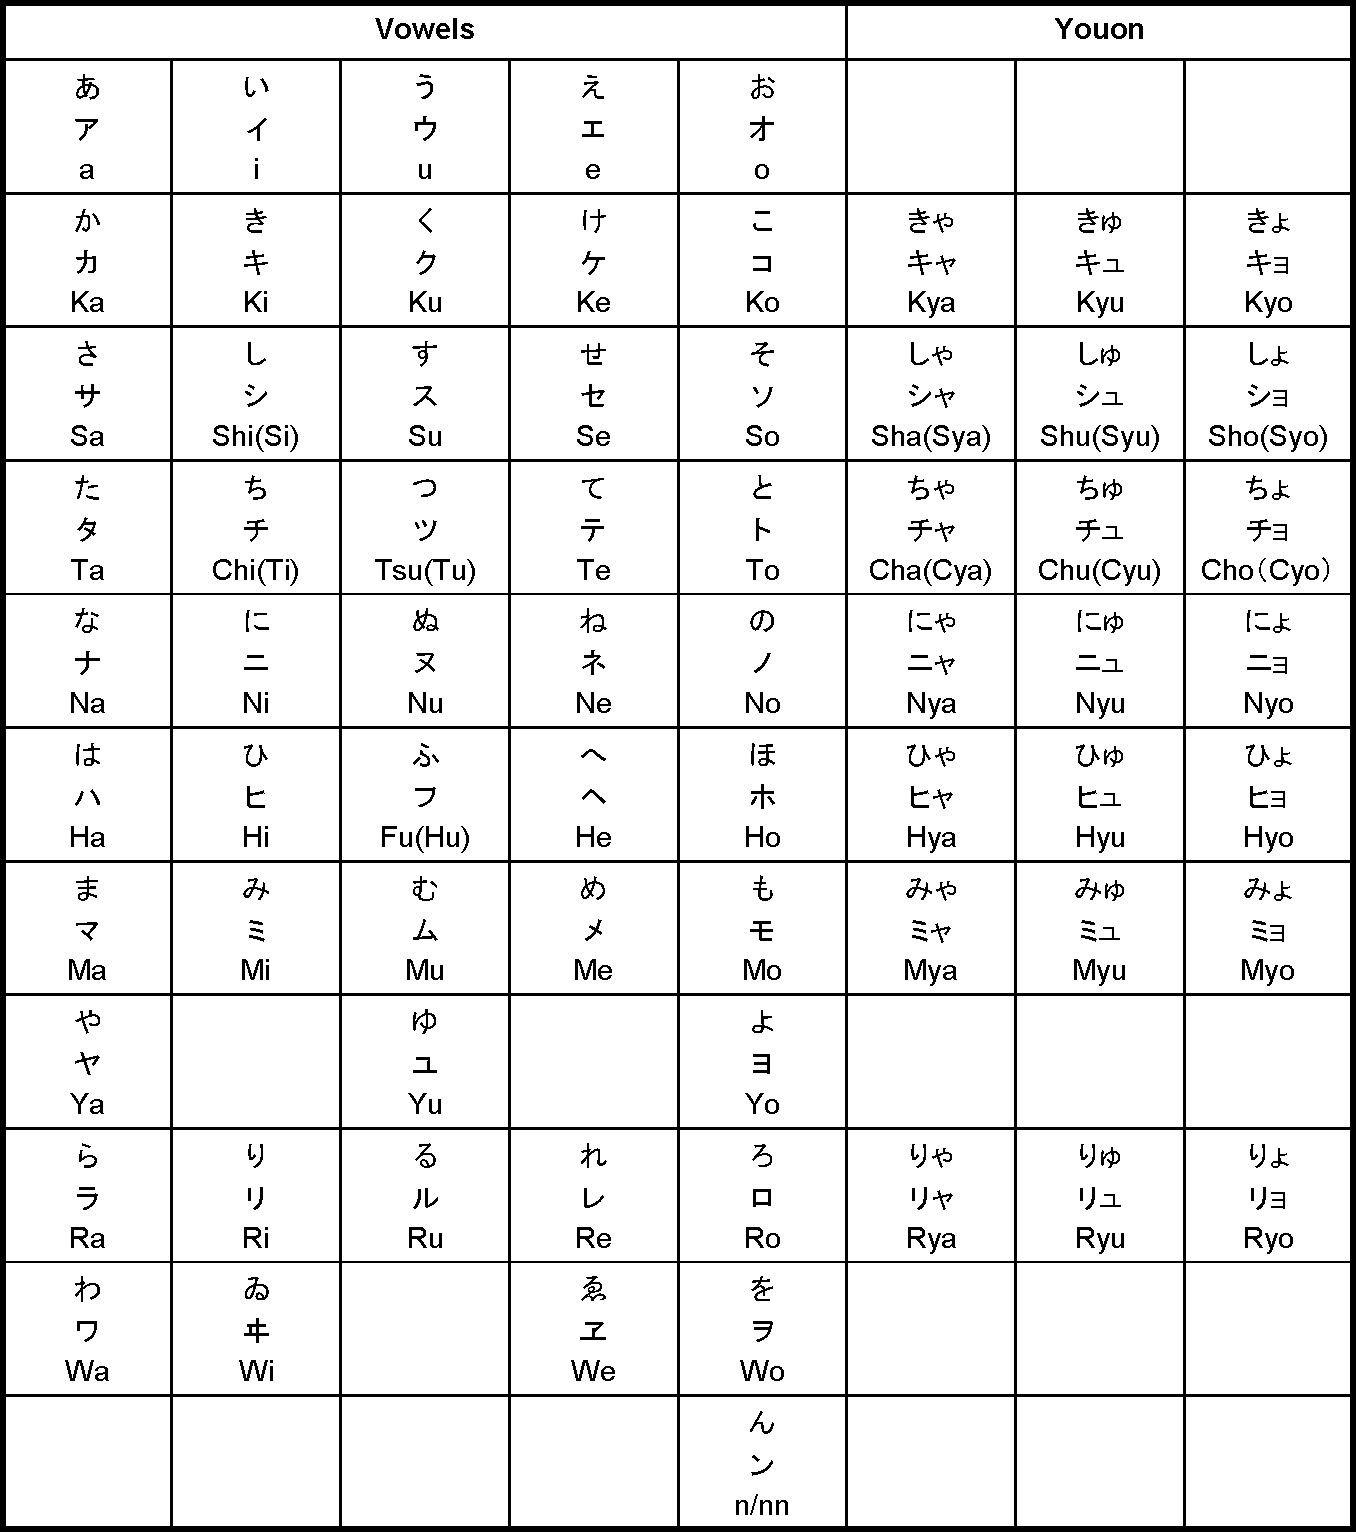
\includegraphics[scale=.114]{material/04japaneseroman}
	\caption{Hiragana, Katakana, lat. Umschrift}
\end{figure}

%\begin{figure}
%\centering
%
%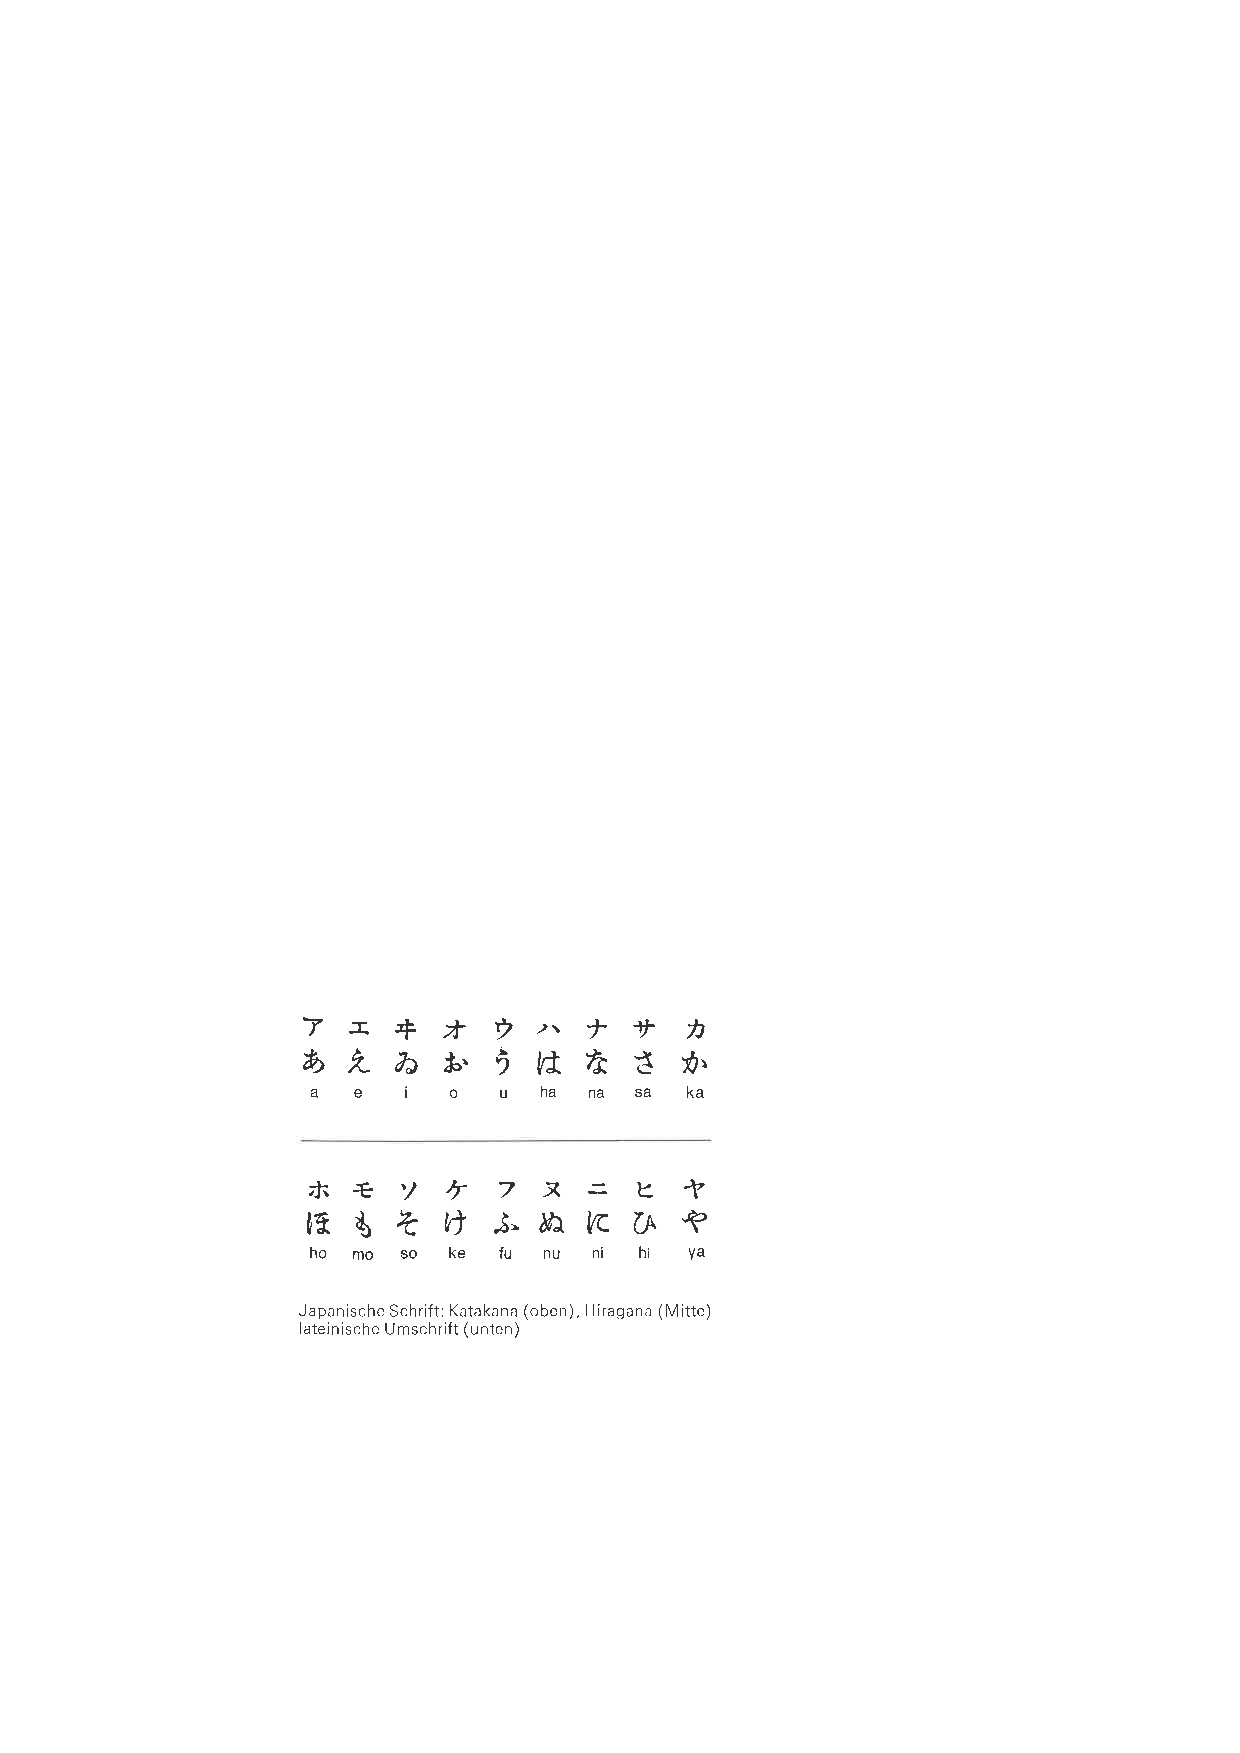
\includegraphics[scale=.45]{material/04JapaneseSyll.pdf}
%\caption{Stiebner; Leonhard (1992): \textit{Bruckmann's Handbuch der Schrift}}
%\end{figure}

\end{minipage}

\end{frame}



%%%%%%%%%%%%%%%%%%%%%%%%%%%%%%%%%%
\begin{frame}
\frametitle{Schriftsysteme}

\begin{itemize}
	\item \textbf{Logographische Schrifttypen}
	
	\begin{itemize}
		\item[]
		\item Bezug von graphischen Einheiten auf Bedeutungseinheiten wie Wörter bzw. Morpheme (kleinste bedeutungstragende Einheiten) 
		\item[]
		\item Bspw. im Chinesischen und in Teilen der ägyptischen Hieroglyphen
		
		
		\end{itemize}
\end{itemize}
		
	\begin{minipage}{.48\textwidth}
	
	\begin{figure}
	\centering
	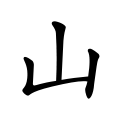
\includegraphics[scale=.45]{material/Chinesemountain-Lee-Sau-Dan}
	\caption[chinese]{\url{https://commons.wikimedia.org/wiki/File:Character\_Shan1\_Trad.svg}; Stand: 05.12.16, Autor: Lee Sau Dan}
	\end{figure}
	
	\end{minipage}\hfill%
	\begin{minipage}{.48\textwidth}
	
	\begin{figure}
	\centering
	
\includegraphics{material/04Hieroglyphen.pdf}
	\caption[Hiero]{Dürscheid (2004): \textit{Einführung in die Schriftlinguistik}}
	\end{figure}
	\end{minipage}
		
\end{frame}



%%%%%%%%%%%%%%%%%%%%%%%%%%%%%%%%%%
\begin{frame}
\frametitle{Schriftsysteme}

\begin{itemize}
	\item Vorteil von phonographischen Schrifttypen:
	
	\begin{itemize}
		\item Mit einem \textbf{eher kleineren Inventar von Zeichen} (20--30) \ras riesige Menge an Wörtern
	\end{itemize}
	
	\item[]
	\item Logographische Schrifttypen benötigen sehr viele Zeichen
	
	\begin{itemize}
		\item Das chinesische Schriftsystem besteht aus ung. 87\,000 Zeichen,\\
                  von denen zwischen 3\,000 und 5\,000 für den Alltag benötigt werden
	\end{itemize}
	
	\item[]
	\item Vorteil von logographischen Zeichen
	\begin{itemize}
		\item Sie können auch von Lesern anderer Dialekte \textbf{einfacher dekodiert} werden.
	\end{itemize}	
\end{itemize}
\end{frame}



%%%%%%%%%%%%%%%%%%%%%%%%%%%%%%%%%%%
\begin{frame}
\frametitle{Schriftsysteme}

Grobe Übersicht der Schrifttypen:
\begin{figure}
\centering
\begin{forest}
MyP edges
	[\textbf{Schrifttypen}
% used to work without tabular
		[\begin{tabular}{@{}l@{}}\textbf{logographischer} \\ Schrifttyp\end{tabular} [[\begin{tabular}{@{}l@{}}Chinesisch \\ Hierogylphen\end{tabular}]]]
		[\begin{tabular}{@{}l@{}}\textbf{phonographischer} \\ Schrifttyp\end{tabular}
			[\begin{tabular}{@{}l@{}}\textbf{alphabetischer} \\ Schrifttyp\end{tabular} [\begin{tabular}{@{}l@{}}Latein \\ Griechisch \\ Russisch\end{tabular}]]
			[\begin{tabular}{@{}l@{}}\textbf{syllabischer} \\ Schrifttyp\end{tabular} [\begin{tabular}{@{}l@{}}Japanisch \\ Koreanisch\end{tabular}]]]]
\end{forest}
\end{figure}

\end{frame}


%%%%%%%%%%%%%%%%%%%%%%%%%%%%%%%%%%
\begin{frame}
\frametitle{Schriftsysteme}

\begin{itemize}
	\item Trotz phonographischer/ alphabetischer Schriftsysteme \ras\\
              sehr verschiedene Schreibung in den unterschiedlichen Sprachen
	\item[]
	\item Unterschiedliche \textbf{graphematische (orthographische) Prinzipien},\\
          die den unterschiedlichen Schreibungen zugrunde liegen
	\item[]
	\item Selten 1-zu-1-Korrespondenz zwischen Phonemen und Graphemen
	
	\begin{itemize}
		\item \textbf{Tiefes System}\\ 
		vs.
		\item \textbf{Flaches System}
	\end{itemize}
\end{itemize}
\end{frame}


%%%%%%%%%%%%%%%%%%%%%%%%%%%%%%%%%%
\begin{frame}
\frametitle{Schriftsysteme}

\begin{itemize}
	\item \textbf{Flaches System}
	
	\begin{itemize}
		\item[]
		\item Sehr gute 1-zu1-Abbildung von Phonemen und Graphemen
		\item[]
		\item Bsp.: Türkisch
		
		\begin{itemize}
			\item[]
			\item 1928: Ersetzung der arabischen Schrift durch die lateinische Schrift
			\item[]
			\item Besonders gute Phonem-Graphem-Abbildung
		\end{itemize}
	\end{itemize}
\end{itemize}
\end{frame}



%%%%%%%%%%%%%%%%%%%%%%%%%%%%%%%%%%
\begin{frame}
\frametitle{Schriftsysteme}

\begin{itemize}
	\item \textbf{Tiefes System}
	
	\begin{itemize}
		\item Abbildung von Phonemen auf Graphemen aber mit Einschränkung
		\item[]
		\item Bsp.: Englisch oder Französisch
		
		\begin{itemize}
			\item Nicht häufig \textbf{reformiert} \ras Starke Abweichung von Aussprache und Schriftform
			\item[]			
			\item Englisch: \textbf{altes} und \textbf{gewachsenes} System mit sehr verschiedenen \textbf{Dialekten} in unterschiedlichen Ländern
			\item[]
			\item Schriftliche Verständigung zwischen den Varietäten ist nur gewährleistet,\\
                          wenn die Phonem-Graphem-Korrespondenz nicht streng durchgezogen wird.
		\end{itemize}
	\end{itemize}
\end{itemize}


\end{frame}



%%%%%%%%%%%%%%%%%%%%%%%%%%%%%%%%%%
\begin{frame}
\frametitle{Schriftsysteme}

%\begin{itemize}
%	\item 

	Türkisch: \ab{dükkan} für \textipa{[dYkkan]}
	
	Spanisch: \ab{negocio} für \textipa{[negoTio]}
	
	Englisch: \ab{business} für \textipa{[bIzn@z]}
	
	Französisch: \ab{boutique} für \textipa{[butik]}
	
\pause	
	
	English: \ab{gh o ti} für \ab{fish} \\
	(\ab{gh} wie in \ab{enough}, \ab{o} wie in \ab{women}, \ab{ti} wie in \ab{nation}
	
%\end{itemize}


\end{frame}



%%%%%%%%%%%%%%%%%%%%%%%%%%%%%%%%%%
\begin{frame}
\frametitle{Schriftsysteme}


\begin{figure}
\centering
	
\includegraphics[scale=.3]{material/04GraphEnglischPGK}
	\caption[EnglischPGK]{https://www.facebook.com/grammarly/photos/a.158139670871698.33824.139729956046003/942699349082389/; Autor: Grammarly; Stand: 05.12.16}
\end{figure}

\end{frame}


%%%%%%%%%%%%%%%%%%%%%%%%%%%%%%%%%%
%%%%%%%%%%%%%%%%%%%%%%%%%%%%%%%%%%
\subsection{Graphematische Prinzipien}
\iftoggle{toc}{
\frame{
\begin{multicols}{2}
\frametitle{~}
	\tableofcontents[currentsection]
\end{multicols}
}
}

%%%%%%%%%%%%%%%%%%%%%%%%%%%%%%%%%%
\begin{frame}
\frametitle{Graphematische Prinzipien}

\begin{itemize}
	\item \textbf{Schrifttyp} bedingt das graphematische System
	\item Daraus ergibt sich die \textbf{Gewichtung} (oder Vorhandensein) weiterer
Prinzipien

	\begin{itemize}
		\item Deutsch \ras alphabetischer Schrifttyp \ras Abbildung von
Phonemen mithilfe von Graphemen
		\item Abbildung von Phonemen auf Grapheme = \textbf{Phonem-Graphem-
Korrespondenz} (PGK)
		\item Weitere Prinzipien:
		
		\begin{itemize}
			\item \textbf{Wortebene}: regelhafte Markierung von Silben, Morphemen und
Bedeutungseinheiten, \dots
			\item[]
			\item \textbf{Satzebene}: regelhafte Groß- und Kleinschreibung, Zusammen- und Getrenntschreibung, \dots
		\end{itemize}
	\end{itemize}
\end{itemize}
\end{frame}



%%%%%%%%%%%%%%%%%%%%%%%%%%%%%%%%%%
\begin{frame}
\frametitle{Graphematische Prinzipien}

\begin{itemize}
	\item Das graphematische System des Deutschen wird von diesen
\textbf{meist regelhaften Prinzipien bestimmt} und dementsprechend
(anschließend) auch \textbf{normiert}, sodass es nur eine einzige
mögliche (normierte) Schreibung für ein Wort gibt.

	\begin{itemize}
		\item[]
		\item Erkundung und Erklärung von Regelmäßigkeiten des Systems \ras
\textbf{Graphematische Herangehensweise}
		\item[]
		\item Anwendung der Regelmäßigkeiten mit einem präskriptiven,
normativen Charakter \ras \textbf{Orthographische Herangehensweise}
	\end{itemize}
\end{itemize}
\end{frame}


%%%%%%%%%%%%%%%%%%%%%%%%%%%%%%%%%%
\begin{frame}
\frametitle{Graphematische Prinzipien}

\begin{itemize}
	\item Graphematische / Orthographische \gqq{Prinzipien}:
	
	\begin{itemize}
		\item Phonographisches Prinzip (nach Phonem-Graphem-Korrespondenzen)
		\item[]
		\item Silbisches Prinzip
		\item[]
		\item Morphologisches Prinzip (Prinzip der Morphemkonstanz)
		\item[]
		\item \gqq{Prinzip} der Homonymiedifferenzierung
		\item[]
		\item Etymologische Schreibung
		\item[]
		\item Ästhetisches \gqq{Prinzip}
		\item[]
		\item Syntaktische Schreibung
	\end{itemize}
\end{itemize}


\end{frame}


%%%%%%%%%%%%%%%%%%%%%%%%%%%%%%%%%%
%%%%%%%%%%%%%%%%%%%%%%%%%%%%%%%%%%
\subsubsection{Phonographisches Prinzip}
%\frame{
%\frametitle{~}
%	\tableofcontents[currentsection]
%}


%%%%%%%%%%%%%%%%%%%%%%%%%%%%%%%%%%
\begin{frame}
\frametitle{Phonographisches Prinzip}

\begin{itemize}
	\item Auch Phonem-Graphem-Korrespondenzen, PGK-Regeln
	\item[]
\pause	
	\item Abbildung von Lauten (Phonen) in Form von Buchstaben \\ vs.
	\item Abbildung von abstrakten, regulären Lautmengen (Phoneme) in
Form von Buchstaben
	\item[]
	\item \textbf{Für}: Phon $\leftrightarrow$ Graphem
	
	\begin{itemize}
		\item[]
		\item Sehr genaue Abbildung
		\item[]
		\item Einfach für den Leser
	\end{itemize}
\end{itemize}


\end{frame}



%%%%%%%%%%%%%%%%%%%%%%%%%%%%%%%%%%
\begin{frame}
\frametitle{Phonographisches Prinzip}

\begin{itemize}
	\item \textbf{Gegen}: Phon $\leftrightarrow$ Graphem
	
	 \begin{itemize}
	 	\item Größeres Inventar an Buchstaben nötig

                   Unterschiedliche Buchstaben (-kombinationen) für \ab{ch}\\
	 	\zB in \ab{ich} und \ab{Buch}
	 	
	 	\item Variabilität der Aussprache in einem Dialekt und in unterschiedlichen Dialekten

		Unterschiedliche Schreibung von \ab{Sport},\\
		\zB \ab{SpoRt}, \ab{Sport}, \ab{Spoat}, \ab{Spocht}
		
		\item \gqq{Verwandtschaft} zwischen Wortformen nicht mehr erkennbar
		
		Unterschiedliche Schreibung von \ab{r}\\
		\zB in \ab{höat} \vs \ab{hören}
		
	 \end{itemize}
\end{itemize}


\end{frame}



%%%%%%%%%%%%%%%%%%%%%%%%%%%%%%%%%%
\begin{frame}
\frametitle{Phonographisches Prinzip}

\begin{itemize}
	\item \textbf{Für}: Phonem $\leftrightarrow$ Graphem
	
	\begin{itemize}
		\item Einheitliche Wiedergabe von komplementärer, freier und
regionaler \textbf{Allophonie}
		\item \textbf{Definition von Graphem} als kleinste
bedeutungsunterscheidende Einheit eines Schriftsystems \ras
Phonem
	\end{itemize}
	
	\item \textbf{Gegen}: Phonem $\leftrightarrow$ Graphem
	
	\begin{itemize}
		\item Für den Leser etwas komplizierter
		
		Wann wird ein \ab{ch} wie in \ab{ich} oder wie in \ab{Buch} ausgesprochen?
		
		\item ABER: Dafür reduziert sich sein Lernaufwand bezüglich der Menge von zu lernenden Buchstaben.	
	\end{itemize}
\end{itemize}


\end{frame}



%%%%%%%%%%%%%%%%%%%%%%%%%%%%%%%%%%
\begin{frame}
\frametitle{Phonographisches Prinzip}

%\begin{itemize}
%	\item 

	\begin{table}
		\centering
		\scalebox{0.8}{
		\begin{tabular}{l c c l c c}
		\textbf{Phonem} & \textbf{einige mögliche} & \textbf{Graphem} & \textbf{Phonem} & \textbf{einige mögliche } & \textbf{Graphem} \\
		& \textbf{Allophone} & & & \textbf{Allophone} & \\ 
		\textipa{/p/} & \textipa{[p], [p\super h]} & \ab{p} & \textipa{/\c{c}/} & \textipa{[\c{c}], [x]} & \ab{ch} \\
		\textipa{/t/} & \textipa{[t], [t\super h]} & \ab{t} & \textipa{/v/} & \textipa{[v]} & \ab{w} \\
		\textipa{/k/} & \textipa{[k], [k\super h]} & \ab{k} & \textipa{/j/} & \textipa{[j]} & \ab{j} \\
		\textipa{/b/} & \textipa{[b], [p]} & \ab{b} & \textipa{/h/} & \textipa{[h]} & \ab{h} \\
		\textipa{/d/} & \textipa{[d], [t]} & \ab{d} & \textipa{/m/} & \textipa{[m]} & \ab{m} \\
		\textipa{/g/} & \textipa{[g], [k]} & \ab{q} & \textipa{/n/} & \textipa{[n]} & \ab{n} \\
		\textipa{/k/+/v/} & [\textsubplus{k}]\textipa{[v]} & \ab{qu} & \textipa{/l/} & \textipa{[l]} & \ab{l} \\
		\textipa{/f/} & \textipa{[f]} & \ab{f} & /\textscr{}/ & [\textscr{}], \textipa{[K], [r], [5]} & \ab{r} \\
		\textipa{/s/} & \textipa{[s]} & \ab{ß} & \textipa{/\t{pf}/} & \textipa{[\t{pf}]} & \ab{pf} \\
		\textipa{/z/} & \textipa{[z]} & \ab{s} & \textipa{/\t{ts}/} & \textipa{[\t{ts}]} & \ab{z} \\
		\textipa{/S/} & \textipa{[S]} & \ab{sch} & \textipa{/\t{tS}/} & \textipa{[\t{tS}]} & \ab{tsch} \\

			
		\end{tabular} 
		}
	\end{table}
%\end{itemize}


\end{frame}



%%%%%%%%%%%%%%%%%%%%%%%%%%%%%%%%%%%
\begin{frame}
\frametitle{Phonographisches Prinzip}

%\begin{itemize}
%	\item 
%\end{itemize}

\begin{table}
	\centering
	\scalebox{0.8}{
	\begin{tabular}{l c l c}
		\textbf{Vokalphonem} & \textbf{Graphem} & \textbf{Vokalphonem} & \textbf{Graphem} \\
		\textbf{(lang und gespannt)} & & \textbf{(kurz und gespannt)} & \\
		\textipa{/i:/} & \ab{ie} & \textipa{/I/} & \ab{i} \\
		\textipa{/y:/} & \ab{ü} & \textipa{/Y/} & \ab{ü} \\
		\textipa{/e:/} & \ab{e} & & \\
		\textipa{/E:/} & \ab{ä} & \textipa {/E/} & \ab{e} \\
		& & \textipa{/@/} & \ab{e} \\
		\textipa{/\o:/} & \ab{ö} & 	\textipa{/\oe/} & \ab{ö} \\
		\textipa{/A:/} & \ab{a} & \textipa{/a/} & \ab{a} \\
		\textipa{/o:/} & \ab{o} & \textipa{/O/} & \ab{o} \\ 
		\textipa{/u:/} & \ab{u} & \textipa{/U/} & \ab{u} \\
	\end{tabular}
	}
\end{table}

\end{frame}



%%%%%%%%%%%%%%%%%%%%%%%%%%%%%%%%%%
\begin{frame}
\frametitle{Phonographisches Prinzip}

%\begin{itemize}
%	\item 
%\end{itemize}

\begin{table}
	\centering
	\scalebox{0.8}{
	\begin{tabular}{c c}
		\textbf{Diphthong} & \textbf{Digraph} \\
		\textipa{/\t{aI}/} & \ab{ei} \\
		\textipa{/\t{aU}/} & \ab{au} \\
		\textipa{/\t{OI}/} & \ab{eu} \\	
	\end{tabular}		
	}
\end{table}

Grapheme mit zwei Buchstaben heißen Digraph, solche mit drei Buchstaben Trigraph, \ldots

\end{frame}

\iftoggle{uebung}{

%%%%%%%%%%%%%%%%%%%%%%%%%%%%%%%%%%
\begin{frame}
\frametitle{Phonographisches Prinzip}

\begin{itemize}
	\item Geben Sie 10 Wörter an, die phonographisch geschrieben werden.
	\item[]	
	\item Wie würden Sie die folgenden Wörter phonographisch schreiben?
		
	\begin{itemize}
		\item Philosophie, Handy, Balkon, Creme, Mutter, Streithahn
	\end{itemize}
	\item[]	
	\item Versuchen Sie, graphematische Regularitäten und Prinzipien zu finden, die die Unterscheidung lang vs.\ kurz bei Vokalen anzeigen. Gibt es Ausnahmen?
		
	\begin{itemize}
		\item Mutter, Mehl, See, Nase, dehnen, gehen, Zoo, Bier, Moor, an, zum, Mann, man, Herbst, Laub, sehr, Bohrer
	\end{itemize}
	
\end{itemize}


\end{frame}

}

%%%%%%%%%%%%%%%%%%%%%%%%%%%%%%%%%%
%%%%%%%%%%%%%%%%%%%%%%%%%%%%%%%%%%
\subsubsection{Silbisches Prinzip}
%\frame{
%\frametitle{~}
%	\tableofcontents[currentsection]
%}


%%%%%%%%%%%%%%%%%%%%%%%%%%%%%%%%%%
\begin{frame}
\frametitle{Silbisches Prinzip}

\begin{itemize}
	\item Auch durch die Lautstruktur zu begründen, aber nicht reine Phonem-Graphem-Beziehungen \ras Bezug auf Vokalqualität/Vokalquantität
	\item In der Graphematik wird (analog zur Silbe in der Phonologie) eine Silbe angenommen:
	
	\begin{itemize}
		\item[]
		\item \textbf{Anfangsrand}: Konsonant(en),\\
		leerer Anfangsrand: \textbf{nackte} Silbe\\
		besetzter Anfangsrand: \textbf{bedeckte} Silbe
		\item[]
		\item \textbf{Silbenkern}: Vokal oder Diphthong
		\item[]
		\item \textbf{Endrand}: Konsonant(en)\\
		leerer Endrand: \textbf{offene} Silbe\\
		besetzter Endrand: \textbf{geschlossene} Silbe
	\end{itemize}
\end{itemize}


\end{frame}



%%%%%%%%%%%%%%%%%%%%%%%%%%%%%%%%%%
\begin{frame}
\frametitle{Silbisches Prinzip}

\begin{itemize}
	\item Vokalqualität und -quantität können phonographisch nicht abgebildet werden (PGK) – aber es gibt Regularitäten auf Silbenebene
	\item[]
	\item Für morphologisch einfache Wörter 
	
	\begin{itemize}
		\item offene Silbe \ras gespannter Vokal: 
		
		  \ea
                  \abe{Klo}, \abe{so}
                  \z
		
		\item geschlossene Silben mit komplexem Endrand
		
		\begin{itemize}
			\item \ras ungespannter Vokal: 
			
			  \ea
                          \abe{Strumpf}, \abe{Bild}
                          \z
			
			\item wenige Ausnahmen: 
			
			  \ea
                          \abe{Mond}, \abe{Keks}, \abe{Obst}
                          \z
			
		\end{itemize}
		\item \dots
	\end{itemize}
\end{itemize}


\end{frame}



%%%%%%%%%%%%%%%%%%%%%%%%%%%%%%%%%%
\begin{frame}
\frametitle{Silbisches Prinzip}

\begin{itemize}
	\item Für morphologisch einfache Wörter:
	
	\begin{itemize}
		\item geschlossene Silben mit einfachem Endrand \ras gespannter und ungespannter Vokal möglich:
		
		  \ea
                  \abe{Beet} - \abe{Bett}, \abe{Bahn} - \abe{Bann}
                  \z
		
		\item Zusätzliche Markierungen möglich, aber nicht immer erforderlich: 
		
		  \ea
                  \abe{an}, \abe{bis}, \abe{rot}, \abe{Hut}
                  \z
		
	\end{itemize}
		
		\item Gespanntheit kann durch \textbf{Verdoppelung des Vokals} \ab{aa}, \ab{ee}, \ab{oo} oder \ab{ie} oder durch ein \ab{h} nach dem Vokal angezeigt werden: 
			
		  \ea
                  \abe{Beet}, \abe{Saal}, \abe{Boot}, \abe{Tier}, \abe{Mehl}
                  \z
		
		\item Ungespanntheit kann durch die \textbf{Verdopplung des Folgekonsonanten} (Geminatenschreibung) angezeigt werden, in zweisilbigen Wörtern sind diese Konsonanten dann ambisyllabisch (im Silbengelenk): 
		
		  \ea
                  \abe{Ebbe}, \abe{Affe}, \abe{Kladde}
                  \z
		
\end{itemize}


\end{frame}


%%%%%%%%%%%%%%%%%%%%%%%%%%%%%%%%%%
\begin{frame}
\frametitle{Silbisches Prinzip}

\begin{itemize}
	\item Zusätzlich zum \ab{ee}
	
	\begin{itemize}
		\item[]
		\item \ab{ee} findet sich auch in offenen Silben, vermutlich weil \ab{e} sowohl für /\textschwa{}/ als auch für \textipa{/e/} steht:
		
		  \ea
                  \ab{\textbf{See}}, \ab{\textbf{Armee}}, \ab{\textbf{Klischee}},
                  \ab{\textbf{Allee}}, \ab{\textbf{Orchidee}}
                  \z
		
	\end{itemize}
\end{itemize}


\end{frame}



%%%%%%%%%%%%%%%%%%%%%%%%%%%%%%%%%%
\begin{frame}
\frametitle{Silbisches Prinzip}

\begin{itemize}
	\item Silbentrennendes \ab{h}
	
	\begin{itemize}
		\item Zwischen zwei \textbf{vokalischen Silbenkernen} \ras zur Markierung der Zweisilbigkeit
		
		
		  \eal
                  \ex \ab{ge-hen}, \ab{Ru-he}, \ab{Mü-he}
		  \ex (oft in Verben) \ab{sehen}, \ab{stehen}
		  \ex (seltener nach Diphthongen) \ab{hauen}, \ab{schauen}
		  \ex (aber nach \ab{ei} beides) \ab{leihen}, \ab{verzeihen}, \ab{schreien}
                  \zl
		
	\end{itemize}
	\item[]
	\item Dehnungs-h vor Sonoranten

	  \ea
          \ab{Mehl}, \ab{Bohrer}
          \z

\end{itemize}


\end{frame}


%%%%%%%%%%%%%%%%%%%%%%%%%%%%%%%%%%
%%%%%%%%%%%%%%%%%%%%%%%%%%%%%%%%%%
\subsubsection{Morphologisches Prinzip}
%\frame{
%\frametitle{~}
%	\tableofcontents[currentsection]
%}


%%%%%%%%%%%%%%%%%%%%%%%%%%%%%%%%%%
\begin{frame}
\frametitle{Morphologisches Prinzip}

\begin{itemize}
	\item Auch Prinzip der Morphemkonstanz, Stammschreibungsprinzip:
	
	\begin{itemize}
		\item[]
		\item Wörter oder Wortformen, die in einer morphologischen Beziehung stehen, werden ähnlich oder gleich geschrieben.
		
		  \eal
                  \ex \ab{Apfel} - \ab{Äpfel}, nicht \ab{Epfel}
		  \ex \ab{Mutter} - \ab{Mütter}, nicht \ab{Mytter}
		  \ex \ab{Ball} - \ab{Bälle}, nicht \ab{Bal} und \ab{Belle}
                  \zl
			 
	\end{itemize}
\end{itemize}


\end{frame}


\iftoggle{uebung}{

%%%%%%%%%%%%%%%%%%%%%%%%%%%%%%%%%%
%%%%%%%%%%%%%%%%%%%%%%%%%%%%%%%%%%
\subsubsection{Übung}
%\frame{
%\frametitle{~}
%	\tableofcontents[currentsection]
%}


%%%%%%%%%%%%%%%%%%%%%%%%%%%%%%%%%%
\begin{frame}
\frametitle{Übung}

\begin{itemize}
	\item Warum schreibt man \ab{dehnen} mit \ab{h}, obwohl das erste \ab{e} in einer offenen Silbe steht und daher nach silbischen Prinzipien sowieso lang gesprochen werden müsste?
	\item[]
	\item Warum schreibt man \ab{mann} und \ab{ball}, obwohl nach silbischen Prinzipien die Geminate einen ambisyllabischen Konsonanten anzeigt?
	\item[]
	\item Warum sind die Wörter \ab{(du) ziehst}, \ab{säubern} und \ab{(er) fällt} Beispiele für morphologisches Schreiben?
	\item[]
	\item Wie müsste man \gqq{phonographisches Schreiben} verstehen, wenn man \ab{Rad} und \ab{König} als Beispiele für das morphologische Prinzip anführt?
\end{itemize}


\end{frame}

}

%%%%%%%%%%%%%%%%%%%%%%%%%%%%%%%%%%
%%%%%%%%%%%%%%%%%%%%%%%%%%%%%%%%%%
\subsubsection{Homonymiedifferenzierungsprinzip}
%\frame{
%\frametitle{~}
%	\tableofcontents[currentsection]
%}


%%%%%%%%%%%%%%%%%%%%%%%%%%%%%%%%%%
\begin{frame}
\frametitle{Homonymiedifferenzierungsprinzip}

\begin{itemize}
	\item Gleichlautende Wörter mit unterschiedlicher Bedeutung werden orthographisch unterschiedlich repräsentiert
	\item[]
	\item Entsprechung:

	  \ea
          Leib – Laib; Seite – Saite; Lied – (Augen)Lid
          \z

	\item Aber:
	
	  \ea
          Kiefer – Kiefer; Bremse – Bremse; Ton – Ton
          \z
	
	\item Möglichkeiten zur Homophonendifferenzierung werden also keineswegs konsequent ausgenutzt.
\end{itemize}


\end{frame}


%%%%%%%%%%%%%%%%%%%%%%%%%%%%%%%%%%
%%%%%%%%%%%%%%%%%%%%%%%%%%%%%%%%%%
\subsubsection{Etymologische Schreibung}
%\frame{
%\frametitle{~}
%	\tableofcontents[currentsection]
%}


%%%%%%%%%%%%%%%%%%%%%%%%%%%%%%%%%%
\begin{frame}
\frametitle{Etymologische Schreibung}

\begin{itemize}
	\item Die Schreibung \gqq{alter} oder entlehnter Wörter bleibt erhalten,\\
          auch wenn sie nicht den aktuellen Schreibprinzipien entspricht.
		
	  \eal
          \ex \ab{wann} statt \ab{wan} (wegen mhd. \ab{wanne})
	  \ex \ab{Creme} statt \ab{Krem}
          \zl

\end{itemize}


\end{frame}


%%%%%%%%%%%%%%%%%%%%%%%%%%%%%%%%%%
%%%%%%%%%%%%%%%%%%%%%%%%%%%%%%%%%%
\subsubsection{Ästhetisches Prinzip}
%\frame{
%\frametitle{~}
%	\tableofcontents[currentsection]
%}


%%%%%%%%%%%%%%%%%%%%%%%%%%%%%%%%%%
\begin{frame}
\frametitle{Ästhetisches Prinzip}

\begin{itemize}
	\item Schreibsilben sollten nicht zu lang und nicht zu kurz sein
	
	  \eal
          \ex \ab{Spiel} statt \ab{Schpiel}
	  \ex \ab{Schwan} statt \ab{Schwahn}
          \zl
	
	\item Verbot von Doppelschreibungen von einigen Vokalgraphemen (\ab{i} und \ab{u} sowie Umlaute) -- teilweise bedingt durch Verwechslungsgefahr
	
	  \ea
          \ab{ii} wie \ab{ü}; \ab{uu} wie \ab{w}
          \z
	
	\item Verbot von Doppelschreibung von Mehrgraphemen wie
	
	  \eal
          \ex \ab{ng} in \ab{Bearbeitungngen}
	  \ex \ab{ch} in \ab{Büchcher} 
	  \ex \ab{sch} in \ab{graphischsch}
          \zl
	
\end{itemize}


\end{frame}


%%%%%%%%%%%%%%%%%%%%%%%%%%%%%%%%%%
%%%%%%%%%%%%%%%%%%%%%%%%%%%%%%%%%%
\subsubsection{Syntaktische Schreibung}
%\frame{
%\frametitle{~}
%	\tableofcontents[currentsection]
%}


%%%%%%%%%%%%%%%%%%%%%%%%%%%%%%%%%%
\begin{frame}
\frametitle{Syntaktisches Prinzip}

\begin{itemize}
	\item Großschreibung für Substantive und Substantivierungen von Adjektiven, Verben, Adverbien und Partikeln (natürlich auch von Satzanfängen und Anrede (\ab{Sie}/\ab{Ihr})
	\item[]
	\item Die Großschreibung von Substantiven gibt es nur in der deutschen (und luxemburgischen) Sprache!
	\item[]
	\item Während der Rechtschreibreform hat man diskutiert, diese abzuschaffen.\\
          Was denken Sie: Was spräche dafür, was dagegen?
\end{itemize}


\end{frame}


\iftoggle{uebung}{

%%%%%%%%%%%%%%%%%%%%%%%%%%%%%%%%%%
%%%%%%%%%%%%%%%%%%%%%%%%%%%%%%%%%%
\subsection{Übungen}
%\frame{
%\frametitle{~}
%	\tableofcontents[currentsection]
%}


%%%%%%%%%%%%%%%%%%%%%%%%%%%%%%%%%%
\begin{frame}
\frametitle{Übungen}

\begin{itemize}
	\item Welche graphematischen Prinzipien (abgesehen von der phonographischen Schreibung) erklären die Schreibung der folgenden Wörter?
	
	  \ea
          \ab{Zimmer}, \ab{Waise}, \ab{Wehen}, \ab{Ruhm}, \ab{Spaß}, \ab{Allee}, \ab{Gras}
          \z

	\item Welche graphematische Funktion erfüllt das \ab{h} in den folgenden Wörtern?
	
	  \ea
          \ab{Nacht}, \ab{Hilfe}, \ab{sehen}, \ab{Mehl}
          \z
		
	\item Wie würden die Wörter \ab{Handy}, \ab{Vasenstück} und \ab{Wannenbad} in phonographischer Schreibung aussehen? Geben Sie zunächst eine phonologische Transkription und schreiben Sie anschließend phonographisch.
\end{itemize}


\end{frame}

}

\iftoggle{hausaufgabe}{
	
	\subsection{Hausaufgabe}
	\iftoggle{toc}{
		\frame{
			\frametitle{~}
			\begin{multicols}{2}
				\tableofcontents[currentsection]
			\end{multicols}	
		}
	}
\begin{frame}%[allowframebreaks]
	\frametitle{Hausaufgabe}
	
\begin{itemize}
	
	\item[1.] Kreuzen Sie die korrekten Aussagen an.
	
	\begin{itemize}
		\item[$\circ$] Die Orthographie ist eine linguistische Teildisziplin, die beschreibt wie man schreibt. Die Graphematik ist dagegen keine Teildisziplin der Linguistik, sondern eine \gqq{willkürliche} (normierende) Festlegung.
		\item[$\circ$] Die Graphematik sollte intuitiv beherrschbar sein und das Lesen und Schreiben vereinfachen.
		\item[$\circ$] Das Wort \ab{kalt} ist eine graphematisch \gqq{nackte} Silbe.
		\item[$\circ$] Es gibt im Deutschen eine eindeutige 1-zu-1-Korrespondenz zwischen Buchstaben und Lauten.
		\item[$\circ$] Das Wort \ab{aufwändig} wird aufgrund des morphologischen Prinzips (auch Prinzip der Schemakonstanz, Stammprinzip oder Verwandtschaftsprinzip) mit \ab{ä} geschrieben (vgl. \ab{Aufwand}).
	\end{itemize}
\end{itemize}
\end{frame}

\begin{frame}
	\begin{itemize}
		\item[2.] Ordnen Sie die graphematischen Prinzipien links den passenden Beispielen für die entsprechenden Prinzipien rechts zu.
		\begin{table}[h!]
			\begin{minipage}{0.45\textwidth}
				\centering
				\begin{tabular}{|l|}
					\hline
					(A) Etymologische Schreibung\\
					\hline
					(B) Homonymievermeidung\\
					\hline
					(C) Morphologisches Prinzip\\
					\hline
					(D) Silbische Prinzip\\
					\hline
					(E) Phonographisches Prinzip\\
					\hline
				\end{tabular}
			\end{minipage}\hfill%
			\begin{minipage}{0.45\textwidth}
				\centering
				\begin{tabular}{|p{0.075\textwidth}|l|}
					\hline
					& Bad, Bäder \\
					\hline
					& gehen \\
					\hline
					& Cello, *Tschello \\
					\hline
					& Wahl, Wal\\
					\hline
					& Flasche \\
					\hline
				\end{tabular}
			\end{minipage}
		\end{table}
	\end{itemize}
\end{frame}

\begin{frame}
	\begin{itemize}
		\item[3.] Betrachten Sie die unten angegebenen Kontexte. Diskutieren Sie kurz anhand dieser Beispiele, ob es sich bei der Groß- und Kleinschreibung des markierten Buchstabens um unterschiedliche Grapheme handeln kann oder nicht.
\eal
			\ex Dieser \underline{W}eg ist sehr steil.
			\ex \underline{W}ege, die ich nicht bewandert habe, gibt es viele.
			\ex Meine Schlüssel sind \underline{w}eg.
			\ex \gqq{\underline{W}eg!}, schrie sie mich an und knallte mir die Tür vor der Nase zu.
			\ex Geh \underline{w}eg!
\zl
	\end{itemize}
\end{frame}

\begin{frame}
	\begin{itemize}
		\item[4.] Erläutern Sie stichpunktartig, welche (graphematische) Funktionen der Buchstabe \gqq{h} in den folgenden Kontexten annimmt:
	\eal
			\ex Ha\underline{h}n:
			\bigskip
			\ex nä\underline{h}en:
			\bigskip
			\ex bein\underline{h}alten:
			\bigskip
			\ex Gesc\underline{h}ichte:
			\bigskip
			\ex Geschic\underline{h}te:
			\bigskip
			\ex Dip\underline{h}thong:
			\bigskip
			\ex Dipht\underline{h}ong:
	\zl
	\end{itemize}
\end{frame}

\begin{frame}
	\begin{itemize}
		\item[5.] Geben Sie die \textbf{phonologische} Transkription, die \textbf{phonetische} Transkription und die \textbf{phonographische} Schreibung (nach der Phonem-Graphem-Korrespondenz) des folgenden Wortes an.
		
		\ea Abstellkammer
		\z
		
	\end{itemize}
\end{frame}
}
%%%%%%%%%%%%%%%%%%%%%% Hausaufgaben Loesung %%%%%%%%%%%%%%%%%%%%%%%%%%

\iftoggle{loesung}{
	
	\subsection{Hausaufgabe}
	\iftoggle{toc}{
		\frame{
			\frametitle{~}
			\begin{multicols}{2}
				\tableofcontents[currentsection]
			\end{multicols}	
		}
	}
	\begin{frame}%[allowframebreaks]
		\frametitle{Hausaufgabe}
		
		\begin{itemize}
			
			\item[1.] Kreuzen Sie die korrekten Aussagen an.
			
			\begin{itemize}
			\item[$\circ$] Die Orthographie ist eine linguistische Teildisziplin, die beschreibt wie man schreibt. Die Graphematik ist dagegen keine Teildisziplin der Linguistik, sondern eine \gqq{willkürliche} (normierende) Festlegung.
			\textcolor{red}{\item[$\checkmark$] Die Graphematik sollte intuitiv beherrschbar sein und das Lesen und Schreiben vereinfachen.}
			\item[$\circ$] Das Wort \ab{kalt} ist eine graphematisch \gqq{nackte} Silbe.
			\item[$\circ$] Es gibt im Deutschen eine eindeutige 1-zu-1-Korrespondenz zwischen Buchstaben und Lauten.
			\textcolor{red}{\item[$\checkmark$] Das Wort \ab{aufwändig} wird aufgrund des morphologischen Prinzips (auch Prinzip der Schemakonstanz, Stammprinzip oder Verwandtschaftsprinzip) mit \ab{ä} geschrieben (vgl. \ab{Aufwand}).}
			\end{itemize}
		\end{itemize}
	\end{frame}
	
	\begin{frame}
		\begin{itemize}
			\item[2.] Ordnen Sie die graphematischen Prinzipien links den passenden Beispielen für die entsprechenden Prinzipien rechts zu.
			\begin{table}[h!]
				\begin{minipage}{0.45\textwidth}
					\centering
					\begin{tabular}{|l|}
						\hline
						(A) Etymologische Schreibung\\
						\hline
						(B) Homonymievermeidung\\
						\hline
						(C) Morphologisches Prinzip\\
						\hline
						(D) Silbische Prinzip\\
						\hline
						(E) Phonographisches Prinzip\\
						\hline
					\end{tabular}
				\end{minipage}\hfill%
				\begin{minipage}{0.45\textwidth}
					\centering
					\begin{tabular}{|p{0.075\textwidth}|l|}
						\hline
						\textcolor{red}{C} & Bad, Bäder \\
						\hline
						\textcolor{red}{D} & gehen \\
						\hline
						\textcolor{red}{A} & Cello, *Tschello \\
						\hline
						\textcolor{red}{B} & Wahl, Wal\\
						\hline
						\textcolor{red}{E} & Flasche \\
						\hline
					\end{tabular}
				\end{minipage}
			\end{table}
		\end{itemize}
	\end{frame}
	
	\begin{frame}
		\begin{itemize}
			\item[3.] Betrachten Sie die unten angegebenen Kontexte. Diskutieren Sie kurz anhand dieser Beispiele, ob es sich bei der Groß- und Kleinschreibung des markierten Buchstabens um unterschiedliche Grapheme handeln kann oder nicht.
			\eal
			\ex Dieser \underline{W}eg ist sehr steil.
			\ex \underline{W}ege, die ich nicht bewandert habe, gibt es viele.
			\ex Meine Schlüssel sind \underline{w}eg.
			\ex \gqq{\underline{W}eg!}, schrie sie mich an und knallte mir die Tür vor der Nase zu.
			\ex Geh \underline{w}eg!
			\zl
			
			\textcolor{red}{
				\item Graphem: Kleinste bedeutungsunterscheidende Einheit im schriftlichen System
				\item \ab{Weg} und \ab{weg} kann als Minimalpaar angesehen werden, und \ab{W} und \ab{w} als unterschiedliche Grapheme, da sie bedeutungsunterscheidend sind. Es gibt darüber hinaus weitere Beispiele, die diese Tendenz zu belegen scheinen \ab{Reisen} \vs \ab{reisen}, \ab{Sie} \vs \ab{sie}, \ab{Gut} \vs \ab{gut}.
				\item Andererseits kann die Großschreibung durch andere Prinzipien bedingt werden (\zB Satzanfang) und verliert somit den bedeutungsunterscheidenden Charakter.
				\item Unter Berücksichtigung \underline{der gegebenen Beispiele} könnte man vermuten das \ab{W} und \ab{w} unterschiedliche Phoneme sind. An sich hat die Groß- und Kleinschreibung aber eine andere Funktion im Schriftsystem des Deutschen!
			}
		\end{itemize}
	\end{frame}
	
	\begin{frame}
		\begin{itemize}
			\item[4.] Erläutern Sie stichpunktartig, welche (graphematische) Funktionen der Buchstabe \gqq{h} in den folgenden Kontexten annimmt:
			\eal
			\ex Ha\underline{h}n: \textcolor{red}{Dehnungs-\ab{h}}
			\bigskip
			\ex nä\underline{h}en: \textcolor{red}{Silbentrennendes \ab{h}}
			\bigskip
			\ex bein\underline{h}alten: \textcolor{red}{Wiedergabe eines Phonems \textipa{[h]} nach den Phonem-Graphem-Korrespondenzen}
			\bigskip
			\ex Gesc\underline{h}ichte: \textcolor{red}{Teil eines Trigraphen \ab{sch} (Achtung! Nicht Teil eines Lauts sondern eines Graphems!)}
			\bigskip
			\ex Geschic\underline{h}te: \textcolor{red}{Teil eines Digraphen \ab{ch} (Achtung! Nicht Teil eines Lauts sondern eines Graphems!)}
			\bigskip
			\ex Dip\underline{h}thong: \textcolor{red}{Teil eines Fremddigraphen \ab{ph}}
			\bigskip
			\ex Dipht\underline{h}ong: \textcolor{red}{Teil eines Fremddigraphen \ab{th}}
			\zl
		\end{itemize}
	\end{frame}
	
	\begin{frame}
		\begin{itemize}
			\item[5.] Geben Sie die \textbf{phonologische} Transkription, die \textbf{phonetische} Transkription und die \textbf{phonographische} Schreibung (nach der Phonem-Graphem-Korrespondenz) des folgenden Wortes an.
			
			\ea Abstellkammer
			\z
			
			\color{red}
			\item[] Phonologisch: \textipa{/ a b S t E l k a m @ \textscr~/}
			\item[] Phonetisch: \textipa{[ P a p S t E l k a m 5 ]}
			\item[] Phonographisch: \ab{ a b sch t e l k a m e r } 
			\item[] Hier erkennt man, dass es sich bei der phonographischen Trankskription um eine Phonem-Graphem-Korrespondenz (und nicht um eine Phon-Graphem-Korrespondenz) handelt.
			
		\end{itemize}
	\end{frame}
}




